\documentclass[12pt, french]{article}

\usepackage{fancyhdr, fancybox, lastpage}
\usepackage[most]{tcolorbox}
\usepackage[a4paper, margin={0.3in, .75in}]{geometry}
\usepackage{wrapfig}
\pagestyle{fancy}
\renewcommand\headrulewidth{1pt}
\renewcommand\footrulewidth{1pt}
\fancyhf{}
\rhead{ \em{Zakaria Haouzan}}
\lhead[C]{\em{2ème année baccalauréat Sciences Mathématiques}}
\chead[C]{}
\rfoot[C]{}
\lfoot[R]{}
\cfoot[]{\em{Page \thepage / \pageref{LastPage}}}


\newtcolorbox{Box2}[2][]{
                lower separated=false,
                colback=white,
colframe=white!20!black,fonttitle=\bfseries,
colbacktitle=white!30!gray,
coltitle=black,
enhanced,
attach boxed title to top left={yshift=-0.1in,xshift=0.15in},
title=#2,#1}


\begin{document}

\begin{center}

\vspace{-2cm}
   \shadowbox {\bf{ Dipôle RL }}
\end{center}

\vspace{-0.5cm}
%%_________________________Exercice ! :"_________________________Exercice
   \begin{Box2}{Exercice 1 : Détermination de l’inductance d’une bobine dans une chaine électronique }
\begin{wrapfigure}{r}{0.22\textwidth}
  \begin{center}
	  \vspace{-0.6cm}
	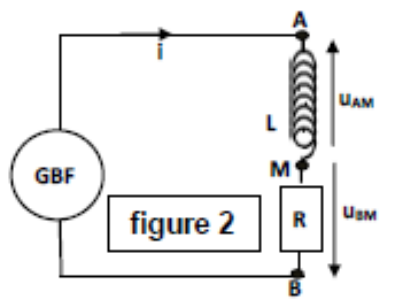
\includegraphics[width=0.22\textwidth]{./img/RL_ex00.png}
  \end{center}
\end{wrapfigure}


On monte en série un conducteur ohmique de résistance $R=2 K \Omega$ et une
bobine d’inductance L et de résistance négligeable, on obtient un dipôle AB On
applique entre les bornes de AB une tension triangulaire à l’aide d’un GBF
(figure 2)

Dans l’intervalle de temps [0 , 2ms], la tension entre les bornes de la bobine
est $u_{AM}=-0,2V$ et la tension $u_{BM}$ entre les bornes du conducteur ohmique est : $u_{BM}=5.10^3 t $ (V)

1. Montrer que la relation entre $u_{AM}$ et $u_{BM}$ est de la forme :
$u_{AM} = -\frac{L}{R}.\frac{du_{BM}}{dt}$

2. Déduire la valeur de l’inductance L de la bobine

   \end{Box2}


%%_________________________Exercice !2 :"_________________________Exercice
\begin{Box2}{Exercice 2 :  Détermination expérimentale de l'inductance L de la bobine }
	\begin{wrapfigure}[10]{r}{0.27\textwidth}
  \begin{center}
	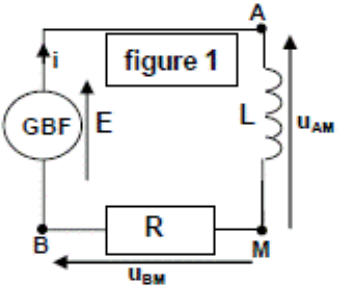
\includegraphics[width=0.22\textwidth]{./img/RL_ex01.png}
	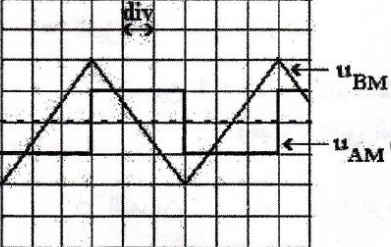
\includegraphics[width=0.27\textwidth]{./img/RL_ex01_1.png}
  \end{center}
\end{wrapfigure}
Pour déterminer expérimentalement l’inductance d’une bobine on réalise le
montage suivant constitué de la bobine (B), du conducteur ohmique de
résistance R

Une bobine (B) d’inductance L et d’un GBF délivrant une tension
rectangulaire (figure 1) On visualise sur un oscilloscope les deux tensions
$u_{AM}(t)$ dans la voie $Y_1$ et $u_{BM(t)}$ dans la voie $Y_2$ on obtient les deux
oscillogrammes de la figure 2

\underline{\textbf{Les données :  }}

\begin{itemize}
	\item La résistance du conducteur ohmique : $R=5.10^3 \Omega$
	\item La sensibilité verticale :  La voie $Y_1$ $S_{V1}=0,2V/div$ , La voie $Y_2$ $S_{V2}=5V/div$
	\item La sensibilité horizontale pour les deux voies : $S_h=1ms/div$

\end{itemize}

1. Recopier le schéma de la figure 1 et montrer comment on
branche l’oscilloscope pour visualiser les deux tensions $u_{AM}$(t) et $u_{BM}(t)$

2. Montrer que l’expression de la tension $u_{AM}$(t) s’écrit : $u_{AM} = -\frac{L}{R}.\frac{du_{BM}}{dt}$

3. Montrer que la valeur de l’induction L de la bobine est $L=0,15H$
\end{Box2}

%%_________________________Exercice ! 3:"_________________________Exercice
\begin{Box2}{Exercice 3 :Etablissement du courant dans le circuit primaire : }
\begin{wrapfigure}{r}{0.12\textwidth}
  \begin{center}
	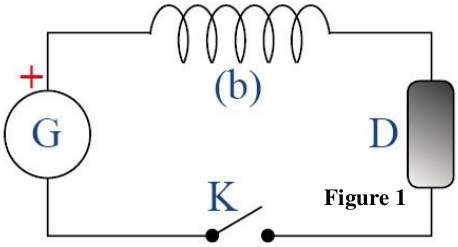
\includegraphics[width=0.12\textwidth]{./img/RL_ex02.png}
  \end{center}
\end{wrapfigure}
	On modélise le circuit primaire par le montage de la figure 2, où :
	
 -  G : Batterie de voiture assimilée à un générateur idéal de
tension continue de f.é.m E=12V.

- (b) : Bobine d’inductance L et de résistance interne r = 1,5 $\Omega$.

- (D) : Un conducteur ohmique équivalent au reste du circuit de
résistance R = 4,5 $\Omega$.

- K : Interrupteur

On ferme l’interrupteur K à l’instant t = 0, le circuit est alors
traversé par un courant électrique i(t).

1. Recopier le circuit de la figure 2 et représenter dessus les tensions en convention récepteur.

2. Montrer que l’équation différentielle vérifiée par le courant i(t) s’écrit sous la forme : $\frac{di}{dt} + \frac{i}{\tau} = A$, en précisant les expressions de $\tau$ et A.

3. Montrer par analyse dimensionnelle que la constante $\tau$ est homogène à un temps.

4. La courbe de la figure 3 représente les variations de
l’intensité du courant en fonction du temps.

4.1. Déterminer graphiquement la valeur de la
constante de temps $\tau$ et celle de l’intensité $I_0$ du
courant en régime permanent.

4.2. En déduire la valeur du coefficient d’inductance L
de la bobine (b).

\end{Box2}

%%_________________________Exercice 4 : _________________________Exercice

\begin{Box2}{Exercice 3 :Etablissement du courant dans le circuit primaire :  }
%\begin{wrapfigure}{r}{0.4\textwidth}
  \begin{center}
	  %\vspace{-0.6cm}
	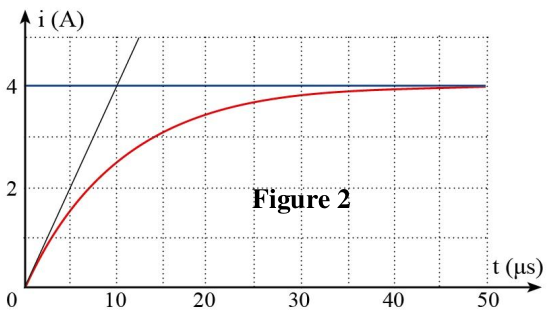
\includegraphics[width=0.33\textwidth]{./img/RL_ex021.png}
  \end{center}
%\end{wrapfigure}


\end{Box2}
%\vspace{2cm}
\begin{center}
\vspace{-0.7cm}
   \Large{ \em{Exercices Supplémentaires}}
\end{center}

\vspace{-0.7cm}

%%_________________________Exercice 5 : _________________________Exercice
\begin{Box2}{Exercice 5 :l’énergie E emmagasinée par la bobine }
	\begin{wrapfigure}[15]{r}{0.27\textwidth}
  \begin{center}
	  %\vspace{-0.6cm}
	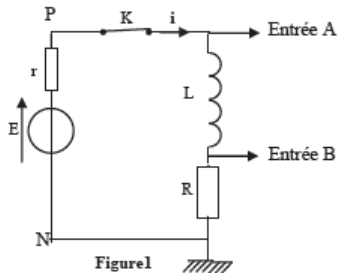
\includegraphics[width=0.2\textwidth]{./img/RLex031.png}
	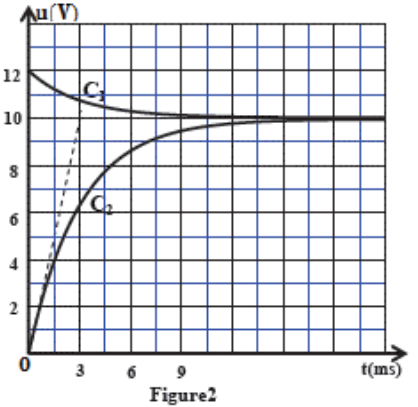
\includegraphics[width=0.27\textwidth]{./img/RL_ex32.png}
  \end{center}
\end{wrapfigure}


On réalise le circuit électrique, schématisé sur la figure 1, qui comporte : 
- Un générateur de tension de f.e.m. E=12V

- Une bobine d’inductance L et de résistance négligeable ;

- Deux conducteurs ohmiques de résistance $R = 40\Omega$

- Un interrupteur K.

On ferme l’interrupteur K à l’instant t=0. Avec un système d’acquisition informatisé, on enregistre les
courbes (C1) et (C2 ) représentant les tensions des voies A et B (voir figure2).

1. Identifier la courbe qui représente la tension $u_R$(t) et celle qui représente $u_{PN}$(t).

2. Déterminer la valeur de $I_P$ l’intensité du courant électrique en régime
permanent.

3. Vérifier que la valeur de la résistance r
du conducteur ohmique est $r=8\Omega$.

4. Etablir l’équation différentielle
régissant l’établissement du courant
i(t)dans le circuit.

5. Trouver les expressions de $A$ et de $\tau$ en
fonction des paramètres du circuit pour
que l’expression $i(t) =A(1- e^{-\frac{t}{\tau}})$, soit solution de
cette équation différentielle.

6. Déterminer la valeur de la constante du temps $\tau$.

7. En déduire la valeur de l’inductance L de la bobine.

8. Trouver l’énergie E emmagasinée par la bobine à l’instant $t = \frac{\tau}{2}$

\end{Box2}
%%_________________________Exercice 6 : _________________________Exercice
%\begin{Box2}{Exercice 6 : échographie}
%%\begin{wrapfigure}{r}{0.2\textwidth}
  %%\begin{center}
	  %%\vspace{-0.6cm}
	%%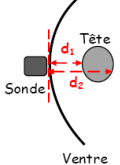
\includegraphics[width=0.2\textwidth]{./img/Exercice6.png}
  %%\end{center}
%%\end{wrapfigure}


%\end{Box2}

\end{document}
